
\chapter{Debug Module (DM)} \label{dm}

\begin{steps}{The Debug Module implements a translation interface between abstract debug
    operations and their specific implementation. It might support the following
    operations:}
\item Give the debugger necessary information about the implementation. (Required)
\item Allow any individual hart to be halted and resumed. (Required)
\item Provide status on which harts are halted. (Required)
\item Provide read and write access to a halted hart's GPRs. (Required)
\item Provide access to a reset signal that allows debugging from the very
    first instruction after reset. (Required)
\item Provide access to other hart registers. (Optional)
\item Provide a Program Buffer to force the hart to execute arbitrary instructions. (Optional)
\item Allow multiple harts to be halted, resumed, and/or reset at the same time. (Optional)
\item Allow direct System Bus Access. (Optional)
\end{steps}

In order to implement memory access, a target must implement either the Program
Buffer or System Bus Access.

A single DM can debug up to 1024 harts.

\section{Debug Module Interface (DMI)} \label{dmi}

The Debug Module is a slave to a bus called the Debug Module Interface (DMI). The
master of the bus is the Debug Transport Module(s).
The Debug Module Interface can be a trivial bus with one master and one slave,
or use a more full-featured bus like TileLink or the AMBA Advanced Peripheral
Bus. The details are left to the system designer.

The DMI uses between 7 and 32 address bits.  It supports read and write
operations.  The bottom of the address space is
used for the DM. Extra space can be used for custom debug devices, other cores,
additional DMs, etc.

The Debug Module is controlled via register accesses to its DMI address space.

\begin{table}[htp]
    \centering
    \caption{Debug Module Interface Address Space}
    \label{tab:header}
    \begin{tabulary}{\textwidth}{|r|L|}
        \hline
        0x00 -- 0x3f & Registers described in Section~\ref{dmdebbus}. \\
        \hline
        0x40 -- 0x5f & This is called the `halt region`.  These 32 addresses
        for 32-bit words provide access to the halt bit for up to 1024 harts.
        If the hart is halted, the bit is 1.  Otherwise
        the bit is 0. The bit for hart 0 is the LSB in the 32-bit word at 0x40.
        The bit for hart 1023 is the MSB in the 32-bit word at 0x5f. \\
        \hline
    \end{tabulary}
\end{table}

\section{Reset Control} \label{reset}

The Debug Module controls a global reset signal, \Fndmreset (non-debug module
reset),
which can reset, or hold in reset, every component in the platform,
except for the Debug Module and Debug
Transport Modules.
Exactly what is affected by this reset is implementation dependent, as long as
it is possible to debug programs from the first instruction executed.
The Debug Module's own state and registers should only be
reset at power-up and while
\Fdmactive in \Rdmcontrol is 0.
The halt state of harts should be
maintained across system reset provided that \Fdmactive is 1,
although trigger CSRs may be cleared.

Due to clock and power domain crossing issues,
it may not be possible to perform arbitrary DMI accesses across
system reset.
While \Fndmreset or any external reset is asserted, the only supported DM
operation is accessing \Rdmcontrol. The behavior of other accesses is
undefined.

\section{Selecting Harts} \label{selectingharts}

Up to 1024 harts can be connected to a single DM. The debugger
selects a hart, and then subsequent halt, resume, reset, and debugging
commands are specific to that hart.

A debugger can enumerate all the harts
attached to the DM by selecting each hart starting from 0
until \Fanynonexistent in \Rdmstatus is 1.

The debugger can discover the mapping between hart indices and
\Rmhartid by using the interface to read \Rmhartid, or by
reading the system's Device Tree.

\subsection {Selecting a Single Hart}

All debug modules must support selecting a single hart.
The debugger can select a hart by writing its index to \Fhartsel.
Hart indexes start at 0 and are contiguous until the final index.

\subsection {Selecting Multiple Harts}

Debug Modules may optionally implement a Hart Array Mask register to allow
selecting multiple harts at once. The debugger can set bits in the hart array mask register
using \Rhawindowsel and \Rhawindow, then apply actions to all selected harts
by setting \Fhasel. If this feature is supported, multiple harts can be
halted, resumed, and reset simultaneously.

Only the actions initiated by \Rdmcontrol can apply to multiple harts
at once, Abstract Commands apply only to the hart selected by
\Fhartsel.

\section{Run Control} \label{runcontrol}

The Debug Module can halt harts and allow them to run again using
the \Rdmcontrol register.
When a debugger wants to halt a single hart it selects it in \Fhartsel
and sets \Fhaltreq, then waits
for \Fallhalted to indicate the hart is halted before clearing \Fhaltreq
to 0. Setting \Fhaltreq has no effect on a hart which is already halted.

To resume, the debugger selects the hart with \Fhartsel,
and sets \Fresumereq. This action sets the hart's
{\tt resumeack} bit to 0. Once the hart has resumed, it
sets its {\tt resumeack} bit to 1. Thus, the
debugger should wait for \Fallresumeack to indicate the
hart has resumed before clearing \Fresumereq to 0.
If a debugger reads \Fallresumeack
and \Fallhalted in the same cycle, the hart must have resumed
and then halted again.

\begin{commentary}
  When waiting for a hart to resume, a debugger should
  examine \Fallresumeack, not \Fallrunning
  or \Fallhalted,
  because the hart may immediately halt again due to
  trigger or step conditions.
\end{commentary}

Setting \Fresumereq on hart which is running
clears {\tt resumeack} but
may cause a hart which halts in the future to immediately
resume. Debuggers should not depend on this behavior and should not
set \Fresumereq for running harts.

To halt or resume multiple harts at the same time, the debugger first
sets the hart's bits in the hart array mask register, then
follows the same procedure but with \Fhasel set to 1.
Depending on the desired operation, the debugger might consider the {\tt any*}
versions of the status instead of {\tt all*}.

When halt or resume is requested, a hart must respond in
less than one second, unless it is unavailable.
(How this is implemented is not further specified. A few
clock cycles will be a more typical latency).

\section{Abstract Commands} \label{abstractcommands}

The DM supports a set of abstract commands, most of which
are optional. Depending on the implementation, the debugger may
be able to perform
some abstract commands even when the selected hart is not halted.
Debuggers can only determine which abstract commands
are supported by a given hart in a given state by attempting them
and then looking at \Fcmderr in \Rabstractcs to see if they were successful.

Debuggers execute abstract commands by writing them to \Rcommand.
Debuggers can determine whether an abstract command is complete by
reading \Fbusy in \Rabstractcs.
If the command takes arguments, the debugger
must write them to the {\tt data} registers before writing to \Rcommand. If a
command returns results, the Debug Module must ensure they are placed
in the {\tt data} registers before \Fbusy is cleared.
Which {\tt data} registers are used for the arguments is
described in Table~\ref{tab:datareg}.  In all cases the least-significant word
is placed in the lowest-numbered {\tt data} register.

\begin{table}[htp]
    \centering
    \caption{Use of Data Registers}
    \label{tab:datareg}
    \begin{tabulary}{\textwidth}{|r|l|l|l|}
        \hline
        XLEN & arg0/return value & arg1 & arg2 \\
        \hline
        32 & \Rdatazero & {\tt data1} & {\tt data2} \\
        \hline
        64 & \Rdatazero, {\tt data1}  & {\tt data2} , {\tt data3} & {\tt data4}, {\tt data5} \\
        \hline
        128 & \Rdatazero-- {\tt data3} & {\tt data4} -- {\tt data7} & {\tt data8} -- {\tt data11} \\
        \hline
    \end{tabulary}
\end{table}

\begin{table}[htp]
    \centering
    \caption{Abstract Register Numbers}
    \label{tab:regno}
    \begin{tabulary}{\textwidth}{|r|l|}
        \hline
        0x0000 -- 0x0fff & CSRs \\
        \hline
        0x1000 -- 0x101f & GPRs \\
        \hline
        0x1020 -- 0x103f & Floating point registers \\
        \hline
        0xc000 -- 0xffff & Reserved for non-standard extensions and internal
        use. \\
        \hline
    \end{tabulary}
\end{table}

\subsection{Abstract Command Listing}

This section describes each of the different abstract commands
and how their fields should be interpreted when
they are written to \Rcommand.

Each abstract command is a 32-bit value. The top 8 bits contain \Fcmdtype which
determines the kind of command. Table~\ref{tab:cmdtype} lists all commands.

\begin{table}[htp]
    \centering
    \caption{Meaning of \Fcmdtype}
    \label{tab:cmdtype}
    \begin{tabulary}{\textwidth}{|r|l|l|l|}
        \hline
        \Fcmdtype & Command & Page \\
        \hline
        0 & Access Register Command & \pageref{access register} \\
        \hline
        1 & Quick Access & \pageref{quick access} \\
        \hline
    \end{tabulary}
\end{table}

\input{abstract_commands.tex}

\begin{figure}
   \centering
   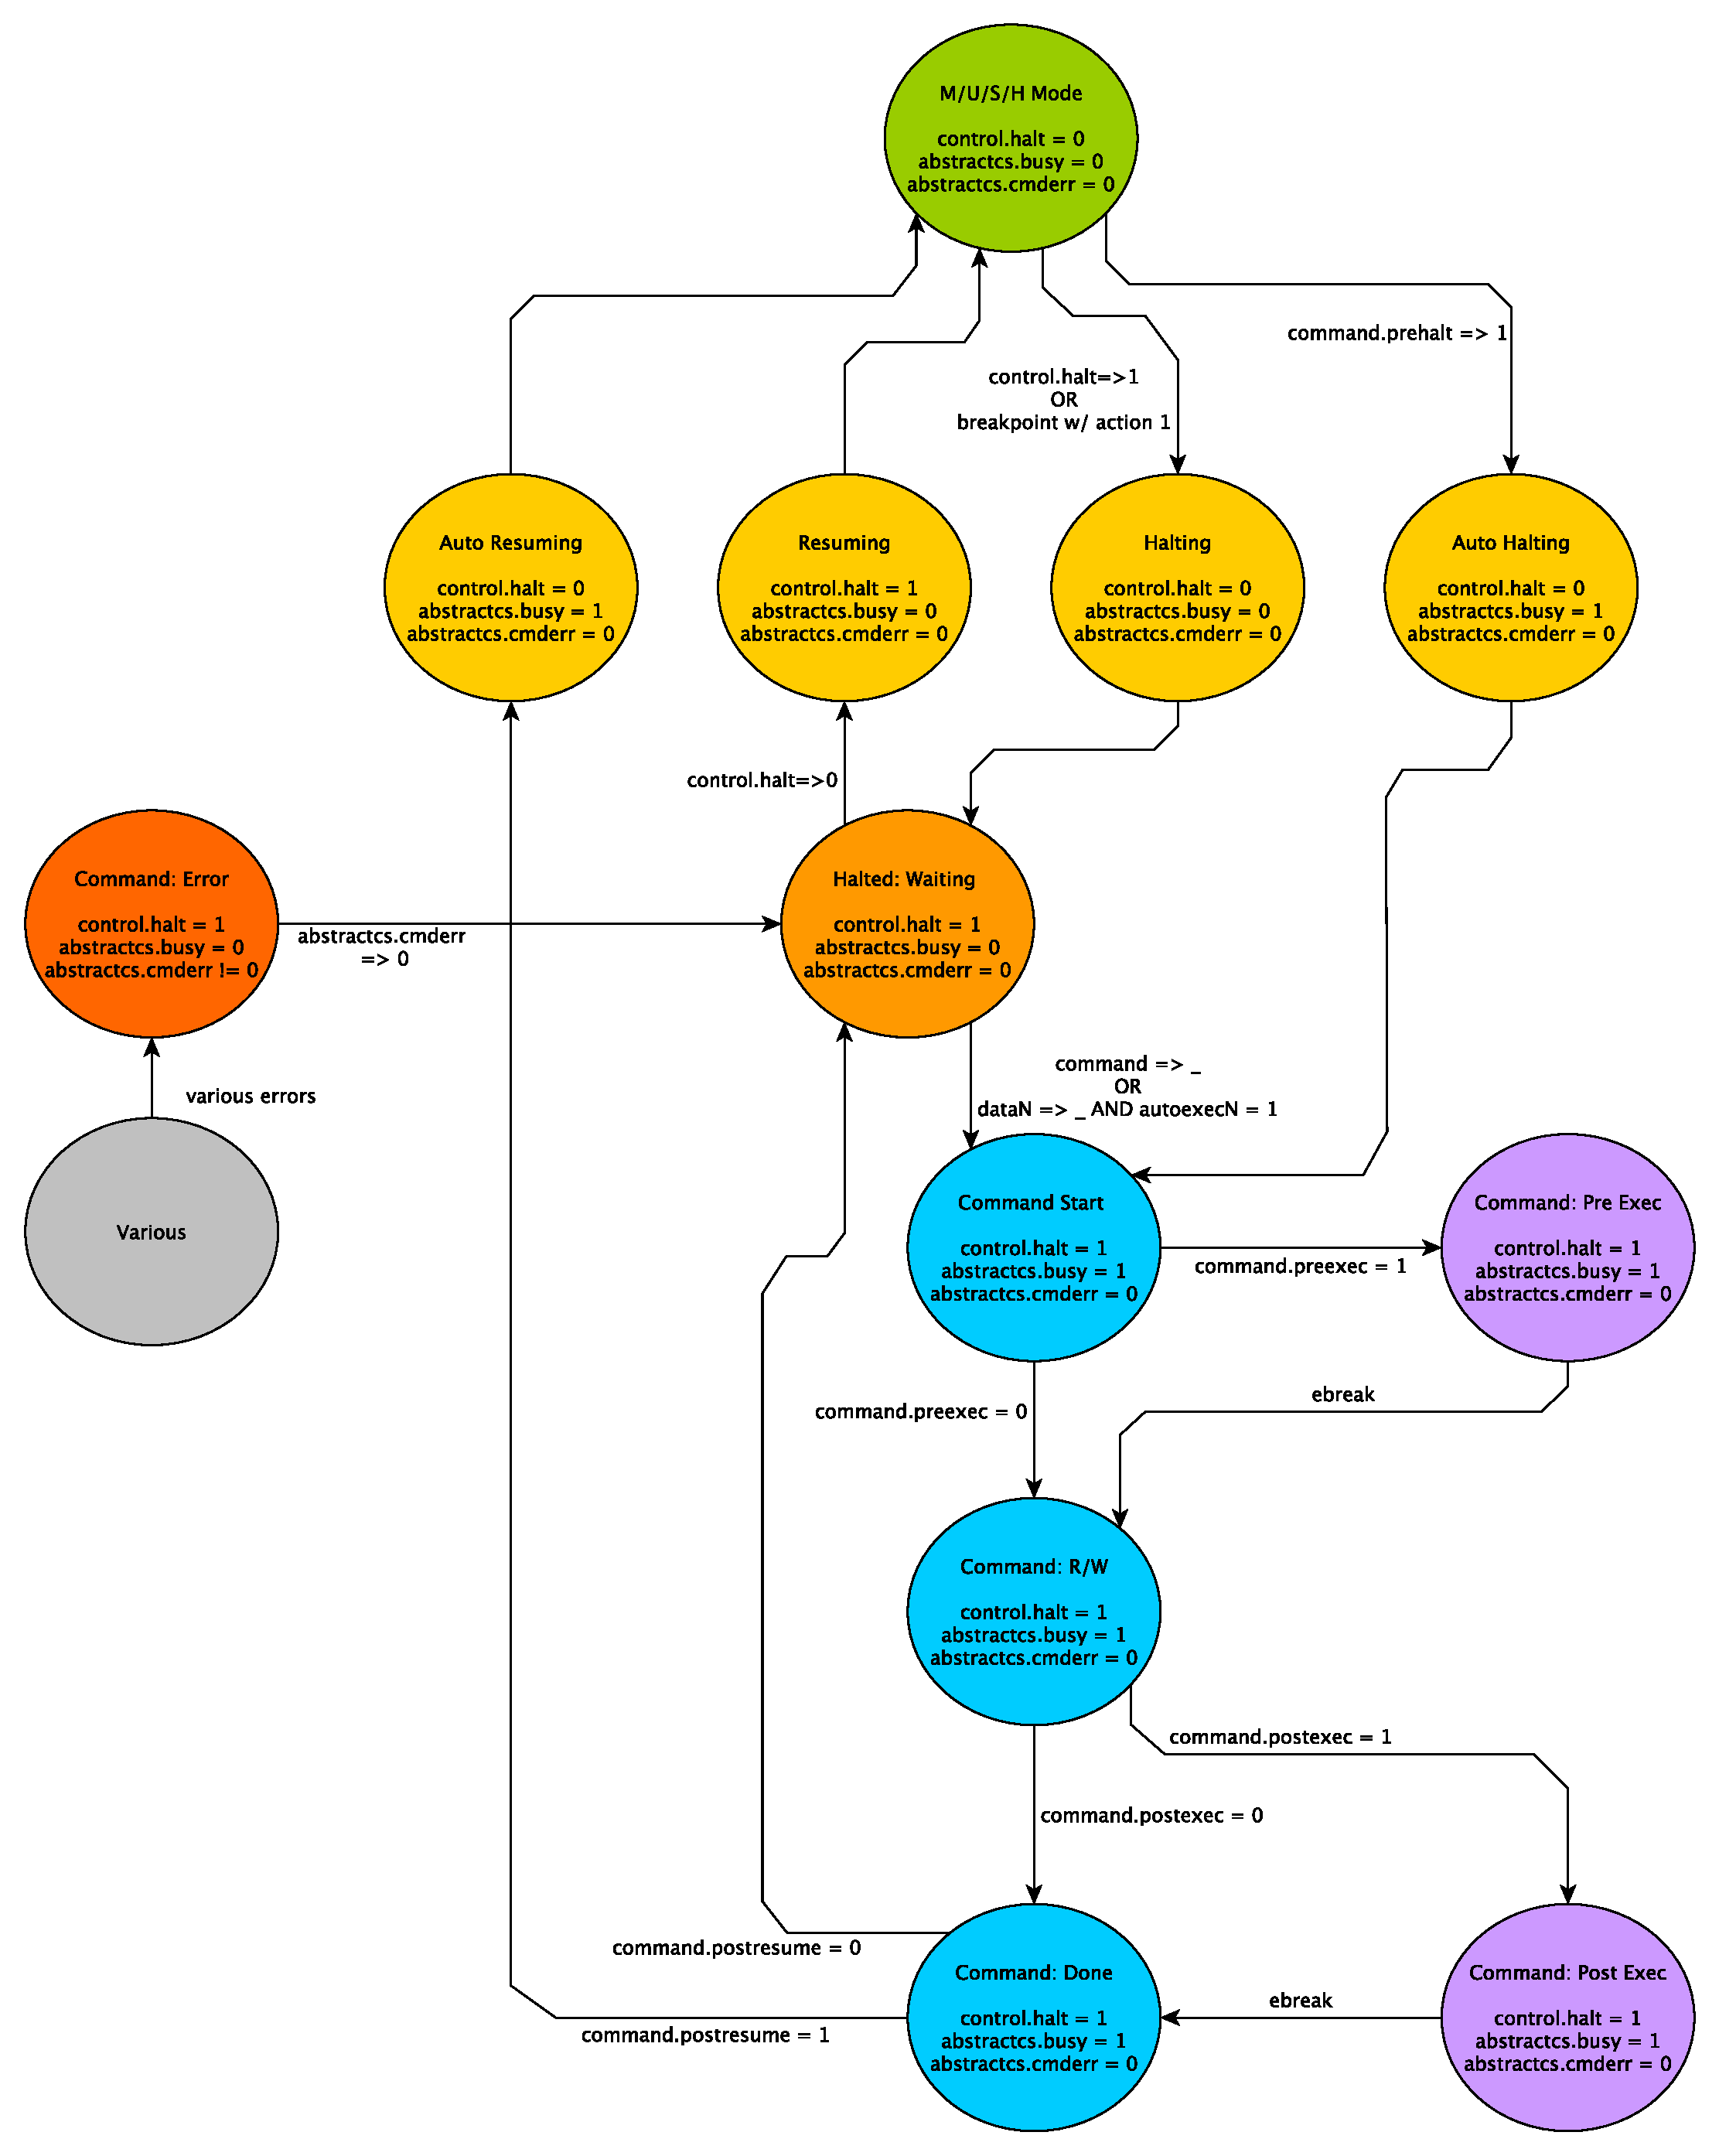
\includegraphics[width=\textwidth]{fig/abstract_commands.pdf}
   \caption[Run/Halt Debug State Machine]{Run/Halt Debug State Machine.
     As only a small amount of state is visibile to the debugger,
     the states and transitions are conceptual.}
   \label{fig:abstract_sm}
\end{figure}

Figure~\ref{fig:abstract_sm} shows a conceptual view of the states
passed through by a hart during run/halt debugging as influenced
by the different fields of \Rdmcontrol, \Rabstractcs, \Rabstractauto, and
\Rcommand.

\section{Program Buffer} \label{programbuffer}

To support executing arbitrary instructions on a halted hart,
a Debug Module can include a 
Program Buffer that a debugger can write small programs to. Systems
that support all necessary functionality using abstract commands
only may choose to omit the Program Buffer.

A debugger can write a small program to the Program Buffer, and then
execute it exactly once with the Access Register Abstract Command,
setting the \Fpostexec bit in \Rcommand.
If \Fprogsize is 1, the Program Buffer may only hold a single instruction.
This can be a 32-bit
instruction, or a compressed instruction in the lower 16 bits accompanied by a
compressed {\tt nop} in the upper 16 bits.  If \Fprogsize is greater than 1,
the debugger can write whatever program it likes, but the program must end with
{\tt ebreak} or {\tt ebreak.c}.

While these programs are executed, the hart does not leave Debug Mode (see
Section~\ref{debugmode}).  If an exception is encountered during execution of
the Program Buffer, no more instructions are executed, the hart remains in Debug
Mode, and \Fcmderr is set to 3 ({\tt exception error}).

Executing the Program Buffer may clobber \Rdpc. If that is the case, it must be
possible to read/write \Rdpc using an abstract command with \Fpostexec not set.
The debugger must attempt to save \Rdpc between halting and
executing a Program Buffer, and then restore \Rdpc before leaving Debug Mode.

\begin{commentary}
    Allowing Program Buffer execution to clobber \Rdpc allows for direct
    implementations that don't have a separate PC register, and do need to use
    the PC when executing the Program Buffer.
\end{commentary}

The Program Buffer may be implemented as RAM which is accessible to the
hart as RAM memory. A debugger can determine if this is the case by executing small
programs that attempt to write relative to \Rpc while executing from the Program Buffer.
If so, the debugger has more flexibility in what it can do with the program buffer.

\section{System Bus Access} \label{systembusaccess}

When a Program Buffer is present, a debugger can access the system bus by having a
RISC-V hart perform the accesses it requires.
A Debug Module may also include a System Bus Access block to provide memory
access without
involving a hart, regardless of whether Program Buffer is implemented.
The System Bus Access block uses physical addresses.

\begin{commentary}
Implementing a System Bus Access block has several benefits even
when a Debug Module also implements a Program Buffer. 
First, it is possible to
access memory in a running system with minimal impact.  Second, it may improve
performance when accessing memory.
Third, it may provide
access to devices that a hart does not have access to.
\end{commentary}

\section{Quick Access}

Depending on the task it is performing, some harts can only be halted very briefly.
There are several mechanisms that allow accessing resources in such a running system
with a minimal impact on the running hart.

First, an implementation may allow some abstract commands to execute without halting the hart.

Second, the Quick Access abstract command can be used to halt a hart, quickly
execute the contents of the Program Buffer, and let the hart run again.
Combined with instructions that allow Program Buffer code to access the
{\tt data} registers, as described in \ref{hartinfo}, this can be used to quickly
perform a memory or register access. For some systems this will be too
intrusive, but many systems that can't be halted can bear an occasional hiccup
of a hundred or less cycles.

Third, if the System Bus Access block is implemented, it can be used while a
hart is running to access system memory.

\section{Security}

To protect intellectual property it may be desirable to lock access to the
Debug Module.  To allow access during a manufacturing process and not
afterwards, a reasonable solution could be to add a fuse bit to the Debug
Module that can be used to be permanently disable it. Since this is technology
specific, it is not further addressed in this spec.

Another option is to allow the DM to be unlocked only by users who have an
access key. A few bits in \Rdmstatus and \Rauthdata can support an arbitrarily
complex authentication mechanism.  When \Fauthenticated is clear, the DM must
not interact with the rest of the platform in any way.

\section{Debug Module DMI Registers} \label{dmdebbus}

When read, unimplemented Debug Module DMI Registers return 0. Writing them has
no effect.

\input{dm_registers.tex}
